% Options for packages loaded elsewhere
\PassOptionsToPackage{unicode}{hyperref}
\PassOptionsToPackage{hyphens}{url}
\PassOptionsToPackage{dvipsnames,svgnames,x11names}{xcolor}
%
\documentclass[
  12pt]{article}

\usepackage{amsmath,amssymb}
\usepackage{iftex}
\ifPDFTeX
  \usepackage[T1]{fontenc}
  \usepackage[utf8]{inputenc}
  \usepackage{textcomp} % provide euro and other symbols
\else % if luatex or xetex
  \usepackage{unicode-math}
  \defaultfontfeatures{Scale=MatchLowercase}
  \defaultfontfeatures[\rmfamily]{Ligatures=TeX,Scale=1}
\fi
\usepackage{lmodern}
\ifPDFTeX\else  
    % xetex/luatex font selection
\fi
% Use upquote if available, for straight quotes in verbatim environments
\IfFileExists{upquote.sty}{\usepackage{upquote}}{}
\IfFileExists{microtype.sty}{% use microtype if available
  \usepackage[]{microtype}
  \UseMicrotypeSet[protrusion]{basicmath} % disable protrusion for tt fonts
}{}
\makeatletter
\@ifundefined{KOMAClassName}{% if non-KOMA class
  \IfFileExists{parskip.sty}{%
    \usepackage{parskip}
  }{% else
    \setlength{\parindent}{0pt}
    \setlength{\parskip}{6pt plus 2pt minus 1pt}}
}{% if KOMA class
  \KOMAoptions{parskip=half}}
\makeatother
\usepackage{xcolor}
\setlength{\emergencystretch}{3em} % prevent overfull lines
\setcounter{secnumdepth}{5}
% Make \paragraph and \subparagraph free-standing
\ifx\paragraph\undefined\else
  \let\oldparagraph\paragraph
  \renewcommand{\paragraph}[1]{\oldparagraph{#1}\mbox{}}
\fi
\ifx\subparagraph\undefined\else
  \let\oldsubparagraph\subparagraph
  \renewcommand{\subparagraph}[1]{\oldsubparagraph{#1}\mbox{}}
\fi


\providecommand{\tightlist}{%
  \setlength{\itemsep}{0pt}\setlength{\parskip}{0pt}}\usepackage{longtable,booktabs,array}
\usepackage{calc} % for calculating minipage widths
% Correct order of tables after \paragraph or \subparagraph
\usepackage{etoolbox}
\makeatletter
\patchcmd\longtable{\par}{\if@noskipsec\mbox{}\fi\par}{}{}
\makeatother
% Allow footnotes in longtable head/foot
\IfFileExists{footnotehyper.sty}{\usepackage{footnotehyper}}{\usepackage{footnote}}
\makesavenoteenv{longtable}
\usepackage{graphicx}
\makeatletter
\def\maxwidth{\ifdim\Gin@nat@width>\linewidth\linewidth\else\Gin@nat@width\fi}
\def\maxheight{\ifdim\Gin@nat@height>\textheight\textheight\else\Gin@nat@height\fi}
\makeatother
% Scale images if necessary, so that they will not overflow the page
% margins by default, and it is still possible to overwrite the defaults
% using explicit options in \includegraphics[width, height, ...]{}
\setkeys{Gin}{width=\maxwidth,height=\maxheight,keepaspectratio}
% Set default figure placement to htbp
\makeatletter
\def\fps@figure{htbp}
\makeatother

\addtolength{\oddsidemargin}{-.5in}%
\addtolength{\evensidemargin}{-1in}%
\addtolength{\textwidth}{1in}%
\addtolength{\textheight}{1.7in}%
\addtolength{\topmargin}{-1in}%

\usepackage{booktabs}
\usepackage{longtable}
\usepackage{array}
\usepackage{multirow}
\usepackage{wrapfig}
\usepackage{float}
\usepackage{colortbl}
\usepackage{pdflscape}
\usepackage{tabu}
\usepackage{threeparttable}
\usepackage{threeparttablex}
\usepackage[normalem]{ulem}
\usepackage{makecell}
\usepackage{xcolor}
\makeatletter
\makeatother
\makeatletter
\makeatother
\makeatletter
\@ifpackageloaded{caption}{}{\usepackage{caption}}
\AtBeginDocument{%
\ifdefined\contentsname
  \renewcommand*\contentsname{Table of contents}
\else
  \newcommand\contentsname{Table of contents}
\fi
\ifdefined\listfigurename
  \renewcommand*\listfigurename{List of Figures}
\else
  \newcommand\listfigurename{List of Figures}
\fi
\ifdefined\listtablename
  \renewcommand*\listtablename{List of Tables}
\else
  \newcommand\listtablename{List of Tables}
\fi
\ifdefined\figurename
  \renewcommand*\figurename{Figure}
\else
  \newcommand\figurename{Figure}
\fi
\ifdefined\tablename
  \renewcommand*\tablename{Table}
\else
  \newcommand\tablename{Table}
\fi
}
\@ifpackageloaded{float}{}{\usepackage{float}}
\floatstyle{ruled}
\@ifundefined{c@chapter}{\newfloat{codelisting}{h}{lop}}{\newfloat{codelisting}{h}{lop}[chapter]}
\floatname{codelisting}{Listing}
\newcommand*\listoflistings{\listof{codelisting}{List of Listings}}
\makeatother
\makeatletter
\@ifpackageloaded{caption}{}{\usepackage{caption}}
\@ifpackageloaded{subcaption}{}{\usepackage{subcaption}}
\makeatother
\makeatletter
\@ifpackageloaded{tcolorbox}{}{\usepackage[skins,breakable]{tcolorbox}}
\makeatother
\makeatletter
\@ifundefined{shadecolor}{\definecolor{shadecolor}{rgb}{.97, .97, .97}}
\makeatother
\makeatletter
\makeatother
\makeatletter
\makeatother
\ifLuaTeX
  \usepackage{selnolig}  % disable illegal ligatures
\fi
\usepackage[]{natbib}
\bibliographystyle{agsm}
\IfFileExists{bookmark.sty}{\usepackage{bookmark}}{\usepackage{hyperref}}
\IfFileExists{xurl.sty}{\usepackage{xurl}}{} % add URL line breaks if available
\urlstyle{same} % disable monospaced font for URLs
\hypersetup{
  pdftitle={Visualising How Non-linear Dimension Reduction Warps Your Data},
  pdfauthor={Jayani P.G. Lakshika; Dianne Cook; Paul Harrison; Michael Lydeamore; Thiyanga S. Talagala},
  pdfkeywords={high-dimensional data, dimension
reduction, triangulation, hexagonal binning, low-dimensional
manifold, manifold learning, tour, data vizualization},
  colorlinks=true,
  linkcolor={blue},
  filecolor={Maroon},
  citecolor={Blue},
  urlcolor={Blue},
  pdfcreator={LaTeX via pandoc}}


\begin{document}


\def\spacingset#1{\renewcommand{\baselinestretch}%
{#1}\small\normalsize} \spacingset{1}

%%%%%%%%%%%%%%%%%%%%%%%%%%%%%%%%%%%%%%%%%%%%%%%%%%%%%%%%%%%%%%%%%%%%%%%%%%%%%%

\title{\bf Visualising How Non-linear Dimension Reduction Warps Your
Data}
\author{
Jayani P.G. Lakshika\\
Econometrics \& Business Statistics, Monash University\\
and\\Dianne Cook\\
Econometrics \& Business Statistics, Monash University\\
and\\Paul Harrison\\
MGBP, BDInstitute, Monash University\\
and\\Michael Lydeamore\\
Econometrics \& Business Statistics, Monash University\\
and\\Thiyanga S. Talagala\\
Statistics, University of Sri Jayewardenepura\\
}
\maketitle

\bigskip
\bigskip
\begin{abstract}
Non-Linear Dimension Reduction (NLDR) techniques have emerged as
powerful tools to visualize high-dimensional data. However, their
complexity and parameter choices may lead to distrustful or misleading
results. To address this challenge, we propose a novel approach that
combines the tour technique with a low-dimensional manifold generated
using NLDR techniques, hexagonal binning, and triangulation. This
integration enables a clear examination of the low-dimensional
representation in the original high-dimensional space. Our approach not
only preserves the advantages of both tours and NLDR but also offers a
more intuitive perception of complex data structures and facilitates
accurate data transformation assessments. The method and example data
sets are available in the \textbf{quollr} R package.
\end{abstract}

\noindent%
{\it Keywords:} high-dimensional data, dimension
reduction, triangulation, hexagonal binning, low-dimensional
manifold, manifold learning, tour, data vizualization
\vfill

\newpage
\spacingset{1} % DON'T change the spacing! (Default 1.9)

\ifdefined\Shaded\renewenvironment{Shaded}{\begin{tcolorbox}[boxrule=0pt, frame hidden, breakable, interior hidden, enhanced, sharp corners, borderline west={3pt}{0pt}{shadecolor}]}{\end{tcolorbox}}\fi

\hypertarget{sec-intro}{%
\section{Introduction}\label{sec-intro}}

High-dimensional (high-D) data is prevalent across various fields, such
as ecology and bioinformatics \citep{Guo2023}, due to advancements in
data collection technologies \citep{Johnstone2009, ayesha2020overview}.
However, visualization of high-D data introduces significant challenges,
because the complexity of visualizing data beyond two dimensions
\citep{Jia2022}. In recent years, interactive and dynamic graphics
systems like \textbf{liminal} \citep{article21} ---which employs
interactive tools like brushing and linking \citep{article58}---and
software tools such as \textbf{XGobi}, \textbf{GGobi} \citep{article60},
\textbf{tourr} \citep{article61}, \textbf{detourr} \citep{article22},
and \textbf{langevitour} \citep{article09}, involving dynamic methods
like tours \citep{Asimov1985}, have played a key role in visualizing
high-D data (data-vis).

To create low-dimensional representations (typically in 2D) (m-vis)
\citep{article59} of high-D data, it is common to apply dimension
reduction (DR) techniques. Approaches for DR involve linear methods such
as principal component analysis (PCA) \citep{Karl1901}, non-linear
methods such as multi-dimensional scaling (MDS) \citep{Torgerson1967}.
In the past decade, many new non-linear dimension reduction (NLDR)
techniques have emerged, such as t-distributed stochastic neighbor
embedding (tSNE) \citep{Laurens2008} and uniform manifold approximation
and projection (UMAP) \citep{Leland2018}. NLDR techniques are the 2D
models of high-D data in our context.

It is important to visualize various non-linear dimensionality reduction
(NLDR) techniques for the same high-D data in order to understand and
find the best representation. After doing so, the 2D models may differ
considerably from each other and may also deviate from the original data
structure in high-dimensional space. Therefore, visualizing the 2D model
in high-D space (m-in-ds) is more useful to answer different types of
questions:

\begin{itemize}
\item
  Is there a best 2D representation of high-D data or are they all
  providing equivalent information? Is there a best parameter choice to
  fit the 2D model? How does the model change when it's parameters
  change?
\item
  How well the does the 2D models capture the data structure? Is the
  model fitting able to capture different data structure like
  non-linear, clustering?
\end{itemize}

If we cannot easily ask and answer these questions, our ability to
understand the models is limited. To find the best 2D model and
parameter choices, a better understanding of the underlying science is
important.

Also, the importance of m-vis along with data-vis has been recognized
and incorporated into interactive software, \textbf{liminal}
\citep{article21}. But the 2D model and high-D visualize side by side
and interactive like brushing and linking connect the data in the two
panels. To address this challenge, we propose a novel approach by
combining the tour technique with a low-dimensional manifold. This
manifold is created through the synergistic use of NLDR techniques,
hexagonal binning, and triangulation. This integration facilitates a
more understanding of the data structure, how well (or how poorly) NLDR
techniques perform.

The outline of this paper is as follows. The
Section~\ref{sec-background} provides an detailed overview of dimension
reduction methods, and tours. Building upon this foundation, the
Section~\ref{sec-methods} delves into the proposed algorithm, its
implementation details, how to tune the model, model summaries, and a
synthetic example to illustrate the functionality of the algorithm.
Subsequently, Section~\ref{sec-applications} showcases applications of
the algorithm on different data sets, particularly in single-cell
RNA-seq data. These applications reveal insights into the performance
and trustworthiness of NLDR algorithms. We analyze the results to
identify situations where NLDR techniques may lead to misleading
interpretations. Finally, \textbf{?@sec-conclusions} concludes by
summarizing the findings and emphasizing the significance of the
proposed approach in tackling the challenges of high-dimensional data
visualization.

\begin{figure}

{\centering 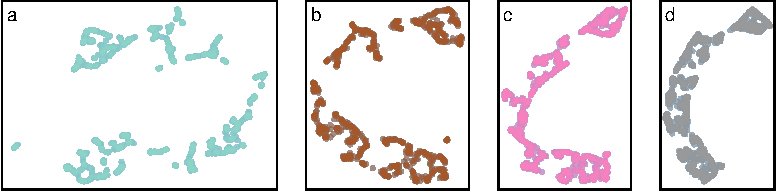
\includegraphics[width=1\textwidth,height=\textheight]{paper_files/figure-pdf/fig-nldervisUMAP-1.pdf}

}

\caption{\label{fig-nldervisUMAP}2D layouts from UMAP applied for the
S-curve data: (a) UMAP (n\_neighbors = 7), (b) UMAP (n\_neighbors = 15),
(c) UMAP (n\_neighbors = 32), (d) UMAP (n\_neighbors = 50). Is there a
best hyperparameter choice in representing UMAP or are they all
providing equivalent information?}

\end{figure}

\hypertarget{sec-background}{%
\section{Background}\label{sec-background}}

\hypertarget{dimension-reduction}{%
\subsection{Dimension Reduction}\label{dimension-reduction}}

Consider the high-D data a rectangular matrix \(X_{n \times p}\), where
\(X_{n \times p} = \begin{bmatrix} \textbf{x}_{1} & \textbf{x}_{2} & \cdots & \textbf{x}_{n}\\ \end{bmatrix}^\top\),
with \(n\) observations in \(p\) dimensions. The objective is to
discover a low-dimensional projection
\(Y_{n \times d} = \begin{bmatrix} \textbf{y}_{1} & \textbf{y}_{2} & \cdots & \textbf{y}_{n}\\ \end{bmatrix}^\top\),
represented as an \(n\) × \(d\) matrix, where \(d \ll p\). The reduction
process seeks to remove noise from the original data set while retaining
essential information.

There are two main categories of dimension reduction techniques: linear
and non-linear methods. Linear techniques involve a linear
transformation of the data, with one popular example being PCA. PCA
performs an eigen-decomposition of the sample covariance matrix to
obtain orthogonal principal components that capture the variance of the
data \citep{Karl1901}.

In contrast, NLDR techniques generate the low-dimensional representation
\(Y\) from the high-dimensional data \(X\), often using pre-processing
techniques like \(k\)-nearest neighbors graph or kernel transformations.
Multidimensional Scaling (MDS) is a class of NLDR methods that aims to
construct an embedding \(Y\) in a low-dimensional space, approximating
the pair-wise distances in \(X\) \citep{Torgerson1967}. Variants of MDS
include non-metric scaling \citep{article62} and Isomap, which estimate
geodesic distances to create the low-dimensional representation
\citep{article63}. Other approaches based on diffusion processes, like
diffusion maps \citep{article64} and the PHATE (Potential of
Heat-diffusion for Affinity-based Trajectory Embedding) algorithm
\citep{article03}, also fall under NLDR methods.

\hypertarget{non-linear-dimension-reduction-techniques}{%
\subsubsection{Non-linear dimension reduction
techniques}\label{non-linear-dimension-reduction-techniques}}

NLDR techniques are crucial for analyzing and displaying
high-dimensional data, where linear approaches may not adequately
capture complexities in relationships between variables
\citep{Johnstone2009}. One of the challenges with NLDR techniques is the
selection and tuning of appropriate hyperparameters \citep{liao2023}.
This process involves finding the suitable combination of
hyperparameters that enhances the performance of the NLDR technique,
considering the characteristics of the dataset and the specific goals of
the analysis.

Additionally, another challenge is lack of reverse mapping. Techniques
like PCA and auto-encoders \citep{article65} provide a way to map back
from the low-dimensional space to the high-D space, facilitating data
reconstruction. However, some NLDR methods, such as tSNE, don't have a
specific way to reconstruct the original data from the low-dimensional
space.

In this article, mainly focus on five NLDR techniques. They are tSNE,
UMAP, PHATE, TriMAP \citep{article02}, and Pairwise Controlled Manifold
Approximation (PaCMAP) \citep{article01}.

Among these, tSNE \citep{Laurens2008} stands out for its ability to
preserve pairwise distances. By minimizing the divergence between
probability distributions in both high and low-dimensional spaces, tSNE
effectively uncovers intricate structures and patterns within the data.
Its application is widespread, particularly in tasks requiring the
visualization of clusters and local relationships. However, achieving
effective results requires careful consideration of hyperparameters,
such as perplexity.

UMAP \citep{Leland2018} is a useful technique for simplifying data while
maintaining both local and overall structures. It builds a fuzzy
topological view by considering nearby data points and then optimizes a
simplified version to match that view. UMAP is known for working well
with different scales of relationships in data and is efficient in
handling large datasets. However, it's important to choose parameters
like neighbors and minimum distance carefully, as they can affect the
results.

Furthermore, PHATE \citep{article03} is great for understanding how
things develop, especially in single-cell genomics. It uses a heat
diffusion process to capture relationships between data points, like
points along a trajectory. While PHATE is excellent for revealing these
developmental structures, it requires careful tuning of its parameters
because of its specialized focus.

Additionally, TriMAP \citep{article02} takes a special approach by
creating a triangulated graph representation of the data. This method is
good at understanding both local and global structures by treating the
data as a network of triangles. TriMAP is powerful in capturing
complicated structures, but it's important to choose parameters
carefully, like deciding how many neighbors to consider.

PaCMAP \citep{article01} is different because it adds supervised
learning to make a 2D representation while keeping the relationships
between pairs of points. It builds a graph using distances between pairs
and then makes the 2D representation better using a customizable loss
function. What's special about PaCMAP is that it can use class labels or
extra information to guide how it makes the 2D representation. This
gives users a way to change how PaCMAP works to fit their needs better.

\begin{figure}

{\centering 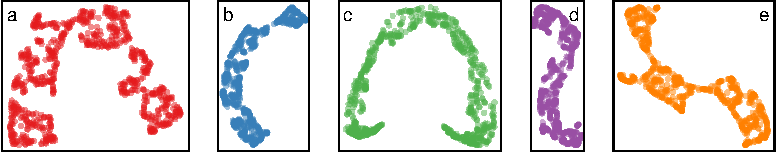
\includegraphics[width=1\textwidth,height=\textheight]{paper_files/figure-pdf/fig-nldervis-1.pdf}

}

\caption{\label{fig-nldervis}2D layouts from different NLDR techniques
applied the same data: (a) tSNE (perplexity = 27), (b) UMAP
(n\_neighbors = 50), (c) PHATE (knn = 5), (d) TriMAP (n\_inliers = 5,
n\_outliers = 4, n\_random = 3), and (e) PaCMAP (n\_neighbors = 10, init
= random, MN\_ratio = 0.9, FP\_ratio = 2). Is there a best
representation of the original data or are they all providing equivalent
information?}

\end{figure}

\hypertarget{linear-overviews-using-tours}{%
\subsection{Linear overviews using
tours}\label{linear-overviews-using-tours}}

A tour is a powerful visualization technique used to explore the shape
and global structure of high-dimensional data by generating a sequence
of projections, typically into two dimensions. There are two main types
of tours: the grand tour \citep{Asimov1985} and the guided tour
\citep{article29}. A grand tour involves randomly selecting new
orthonormal bases, enabling users to understand the structure by
exploring the subspace of d-dimensional projections \citep{Asimov1985}.
In contrast, a guided tour can be employed to generate a sequence of
`interesting' projections based on an index function \citep{article29}.

The process begins with the data matrix \(X\). It generates a sequence
of \(p\) × \(d\) orthonormal projection matrices (bases) \(P_t\),
usually \(d\) is one or two dimensions. For each pair of orthonormal
bases \(P_t\) and \(P_{t+1}\), a geodesic path is interpolated to create
smooth animation between projections. The resulting tour continuously
visualizes the projected data \(Y_t\) = \(XP_t\) as it interpolates
between successive bases.

Furthermore, software like \textbf{langevitour} can visualize both types
of tours, providing flexibility for exploring high-dimensional data with
various objectives. In our context, use grand tour along with the model
to observe how effectively the model captures the underlying structure
of the data.

\hypertarget{sec-methods}{%
\section{Methodology}\label{sec-methods}}

In this paper, we present a novel method that aims to determine the most
effective way to represent high-D data by selecting the best method and
hyperparameter choice. Our approach involves dividing the data set into
two parts: a training set to construct the model and a test set to
generate predictive values and residuals. To implement our approach, we
first use a 2D embedding data set as the initial point. The output of
our algorithm is a tour that displays the model and original data in the
high-dimensional space. A flow chart of the proposed algorithm is shown
in Figure~\ref{fig-meth}. Our algorithm comprises two main phases: (1)
generate the model in the 2D space, and (2) generate the model in the
high-D space. These two phases are described in detail in this section
using UMAP 2D embedding of the S-curve data set, which has seven
dimensions, including four noise dimensions.

\begin{figure}

{\centering 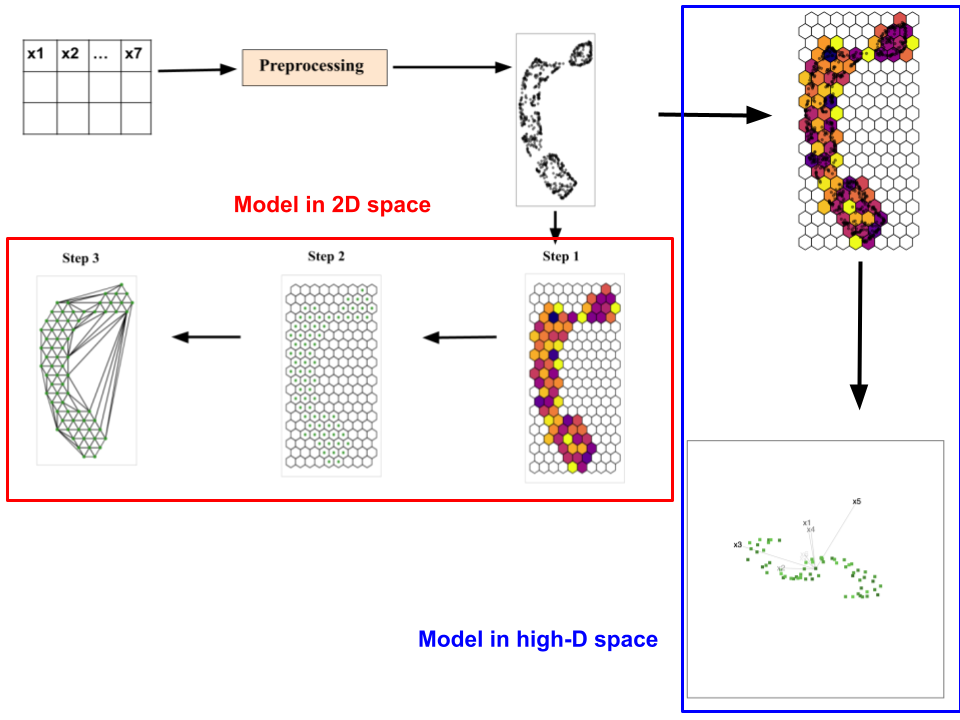
\includegraphics[width=1\textwidth,height=1\textheight]{figures/workflow.png}

}

\caption{\label{fig-meth}A flow diagram detailing the steps taken to
create the low-dimensional manifold in the high dimensional space. There
are two basic phases, one to generate the model in the 2D space, and
other to generate the model in the high-D space.}

\end{figure}

\hypertarget{preprocessing-steps}{%
\subsection{Preprocessing steps}\label{preprocessing-steps}}

In order to reduce the computational complexity associated with
performing NLDR techniques to high-D data, and as a initial step of
noise reduction of high-D data, PCA \citep[\citet{article68},
\citet{article69}]{article67} is applied as a preprocessing step.
Subsequently, the identified principal components, representing
directions of maximum variance, are used to construct the model.

\hypertarget{sec-construct2d}{%
\subsection{Constructing the 2D model}\label{sec-construct2d}}

\textbf{Step 1: Computing the hexagonal grid configuration}

The hexagonal grid, formed through hexagonal binning
\citep[\citet{article66}]{Carr1987}, serves as a type of bivariate
histogram employed to visualize the structure of high-D data. Hexagons,
being one of only three regular polygons capable of tessellating a plane
\citep{Carr2013}, possess both symmetry of nearest neighbors and the
maximum number of sides for a regular tessellation of the plane. This
unique combination makes hexagons more efficient in covering the plane
compared to other regular tessellations. Additionally, hexagons exhibit
lower visual bias when displaying densities, setting them apart from
other regular tessellations \citep{Dan2023}. In our algorithm, hexagonal
binning is used as the initial step of constructing the 2D model and the
total number of bins (\(b\)) is the crucial parameter that defines the
granularity of the hexagonal grid.

\textbf{(a) Determine the number of bins along the x-axis} (\(b_1\))

First, the number of bins along the x-axis (\(b_1\)) is computed using
the relationship between the diameter (\(h\)) and the area (\(A\)) of
regular hexagons (see Equation~\ref{eq-equation3}).

\begin{equation}\protect\hypertarget{eq-equation3}{}{
 \text{A} = \frac{\sqrt{3}}{2}h^2
}\label{eq-equation3}\end{equation}

To construct regular hexagons, \(A = 1\) (see Figure~\ref{fig-binsize})
use as the default setting. Then, the diameter (\(h\)) of the regular
hexagons is calculated (see Equation~\ref{eq-equation4}).

\begin{equation}\protect\hypertarget{eq-equation4}{}{
  \text{h} = \sqrt{\frac{2}{\sqrt{3}}A}
}\label{eq-equation4}\end{equation}

\citet{Carr2013} mentioned about the relationship between the diameter
(\(h\)) of regular hexagons and the height (\(y\)) of the plotting
region. According to our algorithm, the height (\(y\)) of the plotting
region is the the range of 2D embedding component 1 (\(r_1\)) (see
Equation~\ref{eq-equation6}).

\begin{equation}\protect\hypertarget{eq-equation6}{}{
h = \frac{r_1}{b_1}
}\label{eq-equation6}\end{equation}

After rearranging the Equation~\ref{eq-equation6} as
Equation~\ref{eq-equation5}, \(b_1\) is computed. The \(b_1\) value is
rounded up to the nearest whole number to have an integer value.

\begin{equation}\protect\hypertarget{eq-equation5}{}{
b_1 = \frac{r_1}{h}
}\label{eq-equation5}\end{equation}

\textbf{(b) Determine the shape parameter} (\(s\))

In this step, we determine the shape parameter (\(s\)) for the hexagonal
bins, which significantly influences their shape and arrangement within
the grid. The \(s\) in the hexagonal binning algorithm is defined as the
ratio of the height (\(y\)) to the width (\(x\)) of the plotting region
as defined in Equation~\ref{eq-equation1}.

\begin{equation}\protect\hypertarget{eq-equation1}{}{
s = \frac{y}{x}
}\label{eq-equation1}\end{equation}

The shape parameter (\(s\)) of our algorithm is calculated as the ratio
of the ranges of 2D embedding components, where \(r_1\) and \(r_2\)
represent the ranges of 2D embedding components 1 and component 2,
respectively (see Equation~\ref{eq-equation2}).

\begin{equation}\protect\hypertarget{eq-equation2}{}{
s = \frac{r_2}{r_1}
}\label{eq-equation2}\end{equation}

\textbf{(c) Determine the number of bins along the y-axis} (\(b_2\))

Next, the number of bins along the y-axis is computed based on the
number of bins along the x-axis (\(b_1\)) and the shape parameter
(\(s\)) (see Equation~\ref{eq-equation12}) \citep{Carr2013}.

\begin{equation}\protect\hypertarget{eq-equation12}{}{
b_2 = 2 * \left(\frac{(b_1 \times s)}{\sqrt(3)} + 1.5001 \right)
}\label{eq-equation12}\end{equation}

\textbf{(d) Determine the total number of bins} (\(b\))

The total number of bins is determined by multiplying the number of bins
along the x-axis (\(b_1\)) with the number of bins along the y-axis
(\(b_2\)) (see Equation~\ref{eq-equation13}).

\begin{equation}\protect\hypertarget{eq-equation13}{}{
b = b_1 \times b_2
}\label{eq-equation13}\end{equation}

\textbf{Step 2: Obtain bin centroids}

As a result of hexagonal binning for high-D data, all the high-D data
are clustered into hexagons. In this step, the bin centroids
(\(C_k^{(2)} \equiv (C_{ky_1}, C_{ky_2})\)) (see Figure~\ref{fig-meth}
Step 2) are obtained \citep{Carr2013}.

\textbf{Step 3: Triangulate bin centroids}

In this step, the algorithm proceeds to triangulate the hexagonal bin
centroids (see Figure~\ref{fig-meth} Step 3). Triangulation is a
fundamental process in computational geometry and computer graphics that
involves dividing a set of points in a given space into interconnected
triangles \citep{article30}. One common algorithm used for triangulation
is Delaunay triangulation \citep[\citet{article54}]{article26}, where
points are connected in a way that maximizes the minimum angles of the
resulting triangles, leading to a more regular and well-conditioned
triangulation.

Since we are working with the centroids of regular hexagonal bins, the
resulting mesh will predominantly comprise equal-sized regular
triangles. However, the triangulation also helps span any gaps that may
exist between clusters of points, allowing for a more complete and
interconnected representation of the data.

\hypertarget{lifting-the-model-into-high-dimensions}{%
\subsection{Lifting the model into high
dimensions}\label{lifting-the-model-into-high-dimensions}}

\hypertarget{lifting-the-triangular-mesh-points-into-high-dimensions}{%
\subsubsection{Lifting the triangular mesh points into high
dimensions}\label{lifting-the-triangular-mesh-points-into-high-dimensions}}

\textbf{Step1: Cluster 2D points to hexagons}

Expanding upon the information regarding hexagonal binning discussed in
Step 1 of Section~\ref{sec-construct2d}, the primary objective in this
step is to determine the 2D embedding points associated with each
hexagon. As the initial process of hexagonal binning, the 2D points are
clustered into their respective hexagonal bins. By mapping this
information with the hexagonal bin centroids
(\(C_k^{(2)} \equiv (C_{ky_1}, C_{ky_2})\)) that obtained in Step 2 of
the 2D model building (see Section~\ref{sec-construct2d}), we can find
which 2D points are assigned to which data set (see
Figure~\ref{fig-wkhighD} (a)).

\textbf{Step2: Cluster high dimensional points to hexagons}

Following the step 1, the main focus in this step to determine the
corresponding high dimensional points for each hexagon. Every 2D
embedding point serves as a projection of a data point belonging to high
dimensional space. By using this mapping between the high dimensional
data and their corresponding projections, the high dimensional points
allocated to each hexagons are determined (see video linked in
Figure~\ref{fig-wkhighD}).

\textbf{Step3: Compute the mean within hexagon}

Having identified the high-dimensional points associated with hexagons,
the final step involves computing the mean within each hexagonal bin.
This implies calculating the average of the high-dimensional data points
located within each hex bin. These averaged high-dimensional data
points, denoted as \(C_k^{(p)} \equiv (C_{kx_1}, ..., C_{kx_p})\), serve
as the representative coordinates for the hex bin centroids within the
expansive high-dimensional space (see video linked in
Figure~\ref{fig-wkhighD}).

\hypertarget{lifting-the-2d-triangular-mesh-into-high-dimensions}{%
\subsubsection{Lifting the 2D triangular mesh into high
dimensions}\label{lifting-the-2d-triangular-mesh-into-high-dimensions}}

Based on the insights gained in Step 3 of Section~\ref{sec-construct2d},
where connected edges in the 2D triangular mesh were identified, this
step involves lifting these connections into the high dimensions. Having
the mappings of all 2D triangular mesh points into high dimensions, the
points connected in 2D are also connected in high dimensional space (see
video linked in Figure~\ref{fig-wkhighD}).

\begin{figure}

{\centering 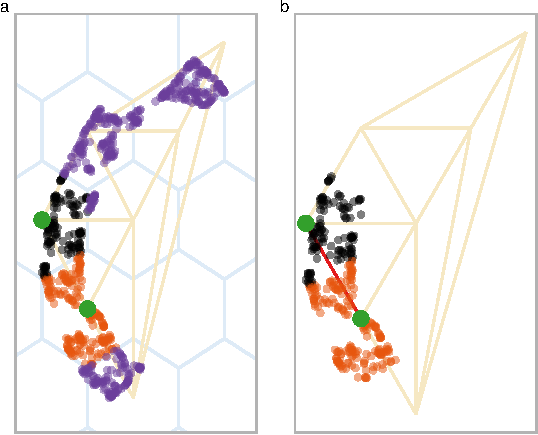
\includegraphics{paper_files/figure-pdf/fig-wkhighD-1.pdf}

}

\caption{\label{fig-wkhighD}How the 2D model lift into high dimensions?
(a) visualize the points and the hexagonal bin centroids related 2nd and
15th hexagons, (b) visualization of the edge connected the 2nd and 15th
hexagons (colored in red) in the triangular mesh. A video of tour
animation is available at \url{https://youtu.be/ffWFVK1UTIc}.}

\end{figure}

\hypertarget{tuning-the-model}{%
\subsection{Tuning the model}\label{tuning-the-model}}

The performance and robustness of our model depend on three key
parameters: (i) the total number of bins (\(b\)), (ii) a benchmark value
used to remove low-density hexagons, and (iii) a benchmark value used to
remove long edges. However, there is no analytical formula to calculate
an appropriate value for these parameters (see Appendix for details on
how default values are calculated). The selection of these parameter
values depends on the model performance computed by Mean Squared Error
(MSE) (see Section~\ref{sec-goodfit}).

\hypertarget{total-number-of-bins}{%
\subsubsection{Total number of bins}\label{total-number-of-bins}}

The number of hexagonal bins in the hexagonal grid has a considerable
impact on the construction of the 2D model. This is because it is the
initial step in building the 2D model. The hexagonal grid with the
chosen total number of bins must be able to capture the structure of the
NLDR data. If the number of bins is too low, the model may not be able
to capture the structure of the NLDR data effectively (see
Figure~\ref{fig-binsize} (a)), while if there are too many bins, it may
result in over-fitting the individual points of the NLDR data (see
Figure~\ref{fig-binsize} (c)). Therefore, it is important to determine
an appropriate number of bins to build an effective model.

Furthermore, the total number of bins is determined by the number of
bins along the x-axis and y-axis (see Equation~\ref{eq-equation13}). To
calculate the effective total number of bins, the minimum and
approximate maximum number of bins along the x-axis are used as
candidate values. The minimum number of bins along the x-axis is \(1\).
The maximum number of bins along the x-axis can be estimated by taking
the square root of the number of NLDR data points. To investigate the
impact of the number of bins on MSE, the analysis is focused on the MSE
for different total numbers of bins. This range encompasses the total
number of bins calculated for the minimum and maximum values of the
number of bins along the x-axis.

Typically, the MSE plot will have a steep slope at the beginning,
indicating that a smaller number of bins causes a larger amount of
error. Then, the slope will gradually decline or level off, indicating
that a higher number of bins generates a smaller error. This MSE plot is
useful in determining the effective number of bins required to construct
the 2D model. Figure~\ref{fig-diagnosticpltScurve} (b) has created a
graph that shows how the Mean Squared Error (MSE) changes depending on
the number of bins assigned in the hexagonal grid for various NLDR
techniques applied to the S-curve data set. As per the rule of thumb
mentioned earlier, the effective number of bins for each NLDR method is
shown in the \textbf{?@tbl-msebinsnldr}. Furthermore,
\textbf{?@fig-modelScurve} shows the 2D models constructed for each NLDR
technique with the selected total number of bins and how the models look
in high-D with original data.

\begin{figure}[H]

{\centering 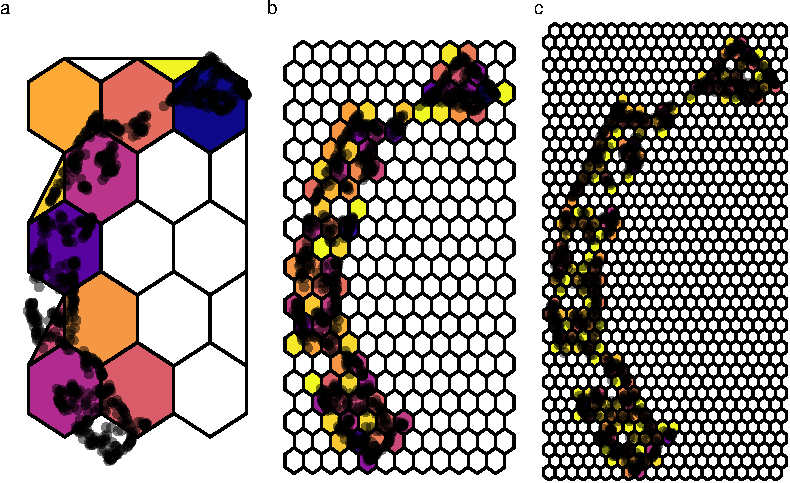
\includegraphics{paper_files/figure-pdf/fig-binsize-1.pdf}

}

\caption{\label{fig-binsize}Hexbin plots from different number of bins
for the \textbf{UMAP} projections of \textbf{S-curve} training data: (a)
b = 32 (4, 8), s = 1.643542, (b) b = 264 (12, 22), s = 1.643542, and (c)
b = 840 (21, 40), s = 1.643542. The hexbins are colored based on the
density of points, with darker colors indicating higher point density
and yellow color representing lower point density within each bin. What
is the number of bins that would be effective in representing
low-dimensional data?}

\end{figure}

\begin{figure}

{\centering 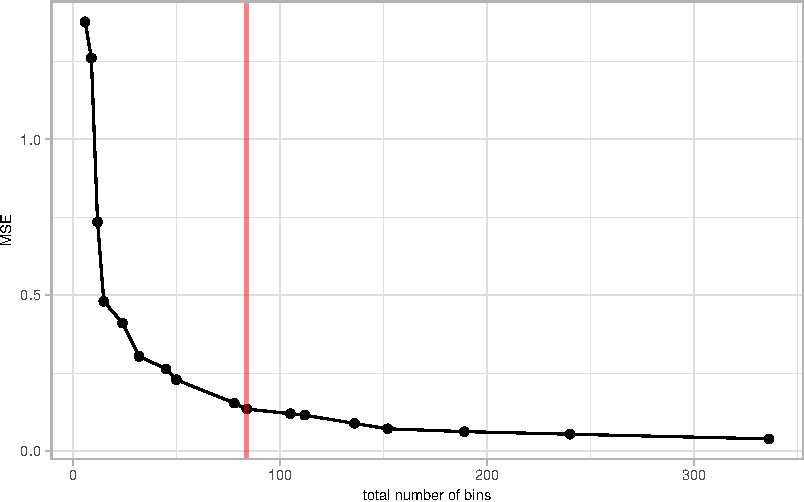
\includegraphics{paper_files/figure-pdf/fig-diagnosticpltScurve-1.pdf}

}

\caption{\label{fig-diagnosticpltScurve}Goodness of fit statistics from
UMAP applied to training S-curve dataset. What is the effective number
of bins in each NLDR technique to create a 2D model? The MSE plot have a
steep slope at the beginning, indicating that a smaller number of bins
causes a larger amount of error. Then, the slope gradually declines or
level off, indicating that a higher number of bins generates a smaller
error. Using the elbow method, when the total number of bins is set to
144, the slope of the Mean Squared Error (MSE) plot experiences a sudden
and noticeable change, resembling an elbow-like shape. This point
indicates that adding less bins does not enough to capture the data
structure.}

\end{figure}

\hypertarget{benchmark-value-to-remove-low-density-hexagons}{%
\subsubsection{Benchmark value to remove low-density
hexagons}\label{benchmark-value-to-remove-low-density-hexagons}}

After setting up the hexagonal grid with an appropriate number of bins,
it is possible that some hexagonal bins may have very few or no data
points within them. To ensure comprehensive coverage of the NLDR data,
it is necessary to select hexagonal bins that have a considerable number
of data points within their hexagons. To achieve this, the standard
number of points within each hexagon is first calculated. This standard
count is obtained by dividing the number of points within each hexagon
by the maximum number of points in the grid (see
Equation~\ref{eq-equationp2}). Next, the bins that have a standard
number of points less than a certain benchmark value are removed. After
removing the hexagons that have insufficient data density, the hexagons
with more substantial data representation are used to construct the 2D
model.

\begin{equation}\protect\hypertarget{eq-equationp2}{}{
\text{standard count} = \frac{\text{count}}{\text{max count}} 
}\label{eq-equationp2}\end{equation}

Furthermore, it is crucial to choose the benchmark value to remove
low-density hexagons carefully. If we remove unnecessary bins, then it
may result in long edges and an uneven 2D model. Therefore, instead of
removing hexagons only identified by the benchmark value, we examine the
standard number of points in the neighboring hexagons of the identified
low-density hexagons. If the neighboring bins also have low counts, then
only those bins will be removed. The other identified bins will be kept
and used for constructing the 2D model along with the high-density bins
(see Appendix for more details).

The benchmark value for removing low-density hexagons has a range of
\(0\) and \(1\). When analyzing how these benchmark values affect model
performance, it's important to observe the change in Mean Squared Error
(MSE) as the benchmark value increases. The MSE exhibits a gradual
increase as the benchmark value progresses from \(0\) to \(1\).
Assessing this rate of increase is crucial. If the increment is not
substantial, the decision might lean towards retaining low-density
hexagons. According to Figure~\ref{fig-diagnosticpltScurvelwd}, the
change in MSE for NLDR techniques is relatively small across different
benchmark values, except for the PHATE method.

Consequently, it is not necessary to remove low-density hexagons when
constructing the 2D model for the S-curve dataset in NLDR techniques,
except for PHATE. While there may be some fluctuations in MSE between
benchmark values of 0 to 1, the absence of significant changes suggests
that maintaining low-density hexagons is preferable. However, to choose
the best selection, it's recommended to examine the benchmark values
around the first local minimum in the MSE curve. However, the MSE for
PHATE fluctuates when benchmark values range between 0 and 1. Therefore,
it is necessary to explore the benchmark values surrounding the first
local minimum to determine an effective benchmark value. There is no
universal rule for selecting a process. As shown in
Figure~\ref{fig-diagnosticpltScurvelwd}, the MSE values for PHATE
fluctuate, and the first local minimum is at \(0\). Therefore, nearby
benchmark values such as \(0.01\), \(0.04\), and \(0.06\) were explored
to identify the best value for preserving the data structure. In this
case, a benchmark value of \(0.06\) was chosen. The resulting 2D model
is shown in \textbf{?@fig-modelScurve} (c), while the video link
provides a visual representation of how the model appears in high-D.

The following steps will help to find a suitable value to remove low
density hexagons:

\begin{enumerate}
\def\labelenumi{\arabic{enumi}.}
\item
  Plot the distribution of the standardized counts
\item
  See the distribution of counts
\item
  Take the first quartile
\end{enumerate}

\begin{figure}[H]

{\centering 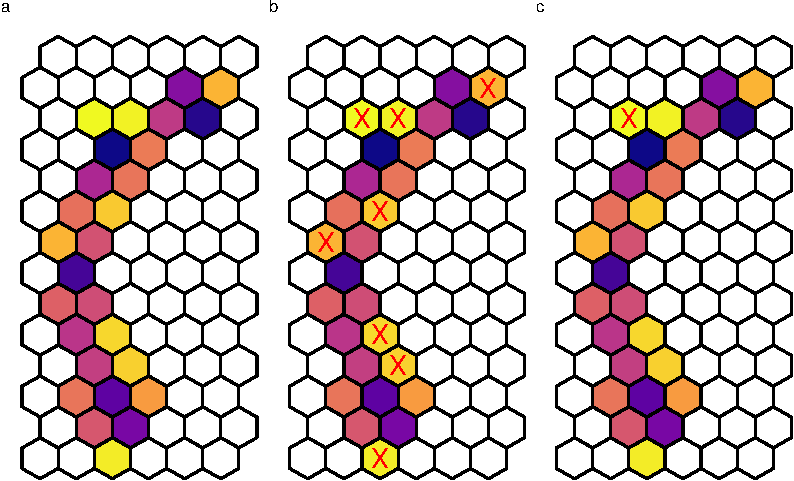
\includegraphics{paper_files/figure-pdf/fig-rmlowdenshex-1.pdf}

}

\caption{\label{fig-rmlowdenshex}Goodness of f}

\end{figure}

\begin{figure}

{\centering 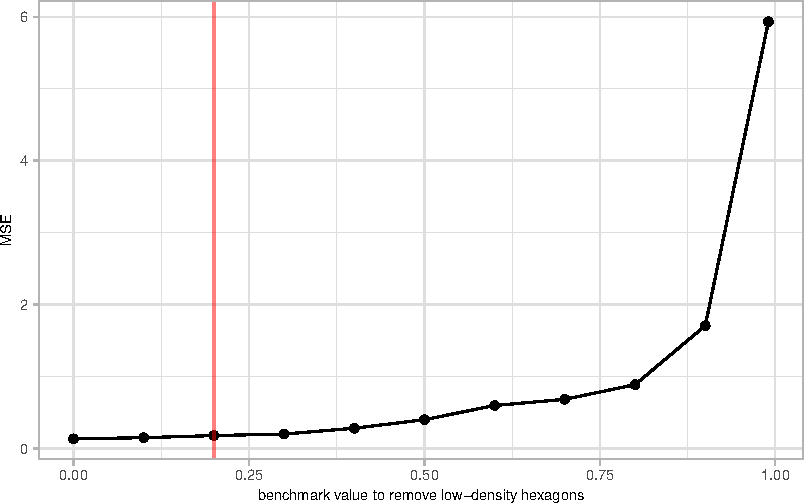
\includegraphics{paper_files/figure-pdf/fig-diagnosticpltScurvelwd-1.pdf}

}

\caption{\label{fig-diagnosticpltScurvelwd}Goodness of fit statistics
from UMAP applied to training S-curve dataset with different benchmark
values to remove the low-density heaxgons. What is the effective
benchmark value to remove the low-density heaxgons? The MSE plot have a
steep slope at the beginning, indicating that a smaller benchmark causes
a small amount of error. Then, the slope gradually increases or level
up, indicating that a higher number of benchmark values generates a
higher error. Using the reverse elbow method, when the benchmark value
is set to 0.2, the slope of the Mean Squared Error (MSE) plot
experiences a sudden and noticeable change, resembling an elbow-like
shape. This point indicates that higher benchmark values remove the
necessary bins as well which lead to distruct the 2D structure.}

\end{figure}

\hypertarget{benchmark-value-to-remove-long-edges}{%
\subsubsection{Benchmark value to remove long
edges}\label{benchmark-value-to-remove-long-edges}}

Achieving a smooth representation in 2D space is crucial, and one factor
influencing this smoothness is the presence of long edges (see
Figure~\ref{fig-modelScurvermlgimp}). These long edges occur when a line
connects points that are distant in the triangular mesh, impacting the
overall smoothness of the mesh.

To investigate the effect of removing long edges on the MSE, we analyzed
the MSE for various benchmark values. Surprisingly, the results
indicated that the MSE remained consistent across different benchmark
values, as shown in \textbf{?@fig-diagnosticpltScurvelgrm}. It's
important to note that edges are defined only in the 2D model and do not
extend to higher dimensions. Consequently, removing edges does not
affect the model in higher dimensions.

There is no definitive rule for determining the benchmark value to
remove long edges. However, we have a method to find a default value
(see Appendix). Adjusting values around this default can help to find
benchmark value to remove long edges, contributing to the construction
of a smoother 2D representation (see
\textbf{?@fig-diagnosticpltScurvelgrm}).

The following steps will help to find a suitable value to remove long
edges:

\begin{enumerate}
\def\labelenumi{\arabic{enumi}.}
\item
  Plot the distribution of the 2D distances
\item
  Find a value which is greater than smallest value
\end{enumerate}

\begin{figure}

{\centering \includegraphics{paper_files/figure-pdf/fig-modelScurverdistcount-1.pdf}

}

\caption{\label{fig-modelScurverdistcount}plots to identify benchmark
values}

\end{figure}

\begin{figure}

{\centering \includegraphics{paper_files/figure-pdf/fig-modelScurvermlgimp-1.pdf}

}

\caption{\label{fig-modelScurvermlgimp}What does the 2D model,
constructed using UMAP (applied to the S-curve dataset), look like in
high dimensions with long edges? (\url{https://youtu.be/pSL_G_n7-fM})
(a) 2D model without removing the long edges, and (b) 2D model with long
edges coloured by red. The default benchmark value is used to identify
long edges.}

\end{figure}

\hypertarget{hexagonal-grid-origin}{%
\subsubsection{Hexagonal grid origin}\label{hexagonal-grid-origin}}

According to \citet{Dan2023}, the hexagonal binning is done by
tessellating the \(xy\) plane over the set (range(\(x\)), range(\(y\)))
(see Figure~\ref{fig-scurveshifthexgridsexp} (b)). In that case, bin
centroids are defined as shown in
Figure~\ref{fig-scurveshifthexgridsexp} (a) with gray colour. Rather
than sticking to the typical hexagonal grid, introducing a meaningful
shift in both the x and y directions presents an opportunity for an
improved 2D model. Therefore, investigating this shift in the hexagonal
grid is an important parameter to consider.

As shown in Figure~\ref{fig-scurveshifthexgrids}, the shifting
influences the distribution of points and number of non-empty bins,
impacting the resulting 2D model. According to
Figure~\ref{fig-diagnosticpltScurvehexbins}, the 2D model with a total
of \(144\) bins applied to S-curve UMAP data does not require any
shifting because the lowest MSE occurs when no shift is introduced.

\begin{figure}

{\centering 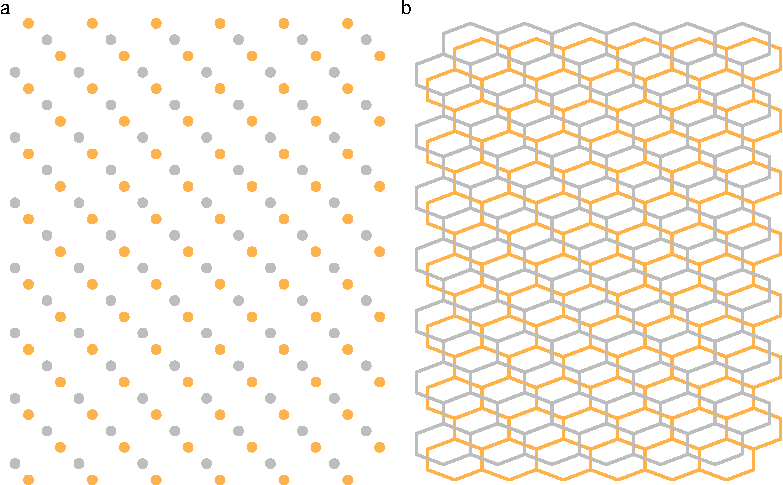
\includegraphics{paper_files/figure-pdf/fig-scurveshifthexgridsexp-1.pdf}

}

\caption{\label{fig-scurveshifthexgridsexp}(a) Visualization of bin
centroids and (b) hexagonal grid, showcasing the configuration before
(colored in gray) and after (colored in light orange) shifting the
starting point by an identical amount applied in both x and y
directions, with a shift value of \(0.537285\).}

\end{figure}

\begin{figure}

{\centering 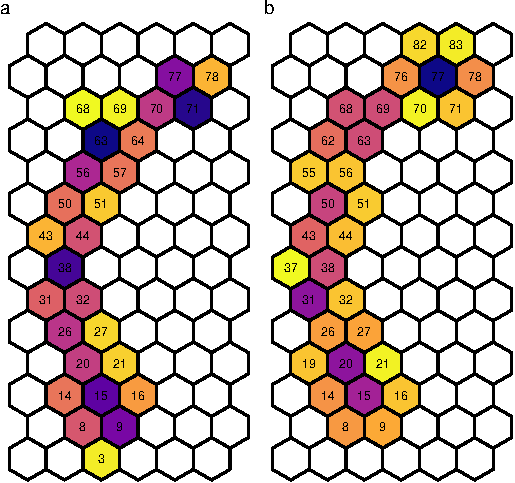
\includegraphics{paper_files/figure-pdf/fig-scurveshifthexgrids-1.pdf}

}

\caption{\label{fig-scurveshifthexgrids}Hexbin plots shows the
distribution of points before and after shifting the starting point of
the hexagonal grid generated for UMAP applied to the training S-curve
dataset. (a) Hexbin plot before shifting, and (b) Hexbin plot after
shifting (identical shift applied in both x and y directions, with a
shift value of \(0.537285\)).}

\end{figure}

\begin{figure}

{\centering \includegraphics{paper_files/figure-pdf/fig-diagnosticpltScurvehexbins-1.pdf}

}

\caption{\label{fig-diagnosticpltScurvehexbins}Goodness of fit
statistics from UMAP applied to training S-curve dataset with different
shift values. In this illustration, an identical shift is applied in
both the x and y directions. The Mean Squared Error (MSE) plot exhibits
a global minimum at \(0\), indicating that no additional shifting is
necessary for the current hexagonal grid to yield a well-fitted model.}

\end{figure}

\hypertarget{sec-summary}{%
\subsection{Model summaries}\label{sec-summary}}

\hypertarget{predicted-values-and-residuals}{%
\subsubsection{Predicted values and
residuals}\label{predicted-values-and-residuals}}

The prediction approach involves employing the K-nearest neighbors (KNN)
algorithm. In this method, which operates as an unsupervised
classification problem, the nearest high-D model point (averaged high-D
point) is identified for the new high-D data point. Once the nearest
high-D model point is identified, its coordinates are used as the
predicted 2D embeddings for the new high-D data point. This step is
particularly valuable due to the limitations of certain NLDR techniques,
like tSNE, which don't provide a straightforward method for predicting
2D embeddings. As a result, our approach presents a solution that can
generate predicted 2D embeddings, irrespective of the NLDR technique
employed, effectively addressing this gap in functionality.

The concept of ``residuals'' is pivotal in evaluating the accuracy of
representing bin centroids in high dimensions. To quantify this
accuracy, we introduce an error metric, which measures the sum of
squared differences between the high-dimensional data (\(x_{ij}\)) and
the predicted bin centroid data in high-dimensional space (\(C_{x_ij}\))
across all bins and dimensions. Mathematically, this error is expressed
as:

\begin{equation}\protect\hypertarget{eq-equation11}{}{
\text{Error} = \sum_{j = 1}^{n}\sum_{i = 1}^{p} (x_{ij} - C_{x_ij})^2
}\label{eq-equation11}\end{equation}

Here, \(n\) represents the number of observations, \(p\) represents the
dimensions, \(x_{ij}\) is the actual high-dimensional data, and
\(C_{x_ij}\) is the predicted bin centroid data in high dimensions.

The error metric outlined above provides valuable insights into the
overall accuracy of our predictive model. By quantifying the squared
deviations between the actual and predicted values across all bins and
dimensions, we gain a comprehensive understanding of how well our method
captures and represents the underlying structure of the data in the
reduced 2D space. This assessment is crucial for evaluating the efficacy
of our NLDR technique in preserving the essential information present in
the original high-dimensional data.

\hypertarget{sec-goodfit}{%
\subsubsection{Goodness of fit statistics}\label{sec-goodfit}}

Moving on to the assessment of prediction accuracy, we calculate the
Mean Squared Error (MSE). The MSE helps measure the average squared
differences between the actual high-dimensional data (\(x_{ij}\)) and
the predicted bin centroid data in high-D (\(C_{x_ij}\)) values across
all bins. Mathematically, this is expressed as:

\begin{equation}\protect\hypertarget{eq-equation9}{}{
\text{MSE} = \sum_{j = 1}^{n} \frac{\sum_{i = 1}^{p} (x_{ij} - C_{x_ij})^2}{n}
}\label{eq-equation9}\end{equation}

Here, \(b'\) signifies the total number of bins without empty bins,
\(p\) denotes the number of dimensions in the high-dimensional data, and
\(n\) represents the number of observations.

Additionally, we gauge the model's performance using the Akaike
Information Criterion (AIC), calculated by the formula:

\begin{equation}\protect\hypertarget{eq-equation10}{}{
\text{AIC} = 2b'p + np * log(\text{MSE})
}\label{eq-equation10}\end{equation}

These metrics, MSE and AIC, collectively offer valuable insights into
the model's predictive performance, considering both accuracy and
complexity in the predictions.

\hypertarget{sec-simpleex}{%
\subsection{Simulated data example}\label{sec-simpleex}}

In this section, we showcase the effectiveness of our methodology using
simulated data. The dataset comprises five spherical Gaussian clusters
in 4-\(d\), with each cluster containing an equal number of points and
consistent within variation.

In the 2D representations created by all NLDR techniques, as shown in
Figure~\ref{fig-nldervis5Gau}, except for PHATE, there are five distinct
clusters. In tSNE, these five clusters are closely located to each other
(see Figure~\ref{fig-nldervis5Gau} (a)). However, in PHATE, two clusters
are closely positioned, while the other three are more distant (see
Figure~\ref{fig-nldervis5Gau} (c)). In PaCMAP, one cluster is at the
center, and the remaining four are positioned in four different
directions (see Figure~\ref{fig-nldervis5Gau} (e)). In TriMAP, two
clusters are close, although not as close as in PHATE, and the other
three are well-separated (see Figure~\ref{fig-nldervis5Gau} (d)). In
UMAP, all clusters are arranged in a parallel manner, with three in one
line and the other two in a separate line (see
Figure~\ref{fig-nldervis5Gau} (b)).

Visualizing the models alongside the original high-D data provides
insights into how different techniques capture the underlying clustering
structure. The tSNE model exhibits five well-separated clusters,
effectively preserving both local and global structures (see video link
of Figure~\ref{fig-modelfiveGau} (a)). UMAP, on the other hand, also
presents five distinct clusters but with a more flattened surface
appearance (see video link of Figure~\ref{fig-modelfiveGau} (b)). The
PHATE model shows five separated clusters resembling triangles or
partial triangles but struggles to capture local structures (see video
link of Figure~\ref{fig-modelfiveGau} (c)). TriMAP and PaCMAP both
display five well-separated clusters with flat surfaces, each capturing
within-cluster variation to varying extents. Despite the various 2D
representations, all NLDR techniques preserve the global structure (see
video link of Figure~\ref{fig-modelfiveGau} (d), (e) respectively).
However, tSNE, effectively capture both local and global structures, as
indicated by lower AIC values in Figure~\ref{fig-diagnosticpltGau} (a).

\begin{figure}

{\centering 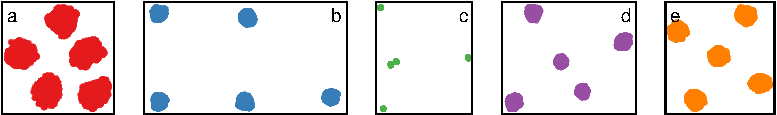
\includegraphics[width=1\textwidth,height=\textheight]{paper_files/figure-pdf/fig-nldervis5Gau-1.pdf}

}

\caption{\label{fig-nldervis5Gau}2D layouts from different NLDR
techniques applied the same data: (a) tSNE (perplexity = 61), (b) UMAP
(n\_neighbors = 15), (c) PHATE (knn = 5), (d) TriMAP (n\_inliers = 5,
n\_outliers = 4, n\_random = 3), and (e) PaCMAP (n\_neighbors = 10, init
= random, MN\_ratio = 0.9, FP\_ratio = 2). Is there a best
representation of the original data or are they all providing equivalent
information?}

\end{figure}

\begin{figure}

{\centering 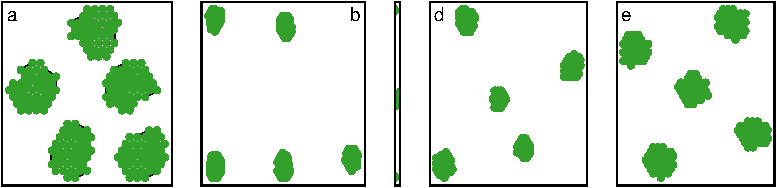
\includegraphics[width=1\textwidth,height=\textheight]{paper_files/figure-pdf/fig-modelfiveGau-1.pdf}

}

\caption{\label{fig-modelfiveGau}Is there a best model to represent the
original data in 2D space or are they all providing equivalent
information?, (a) Model in the 2D space with tSNE
(\url{https://youtu.be/x5VPB-wOLm4}), (b) Model in the 2D space with
UMAP (\url{https://youtu.be/Cm1dW6iLyHQ}), (c) Model in the 2D space
with PHATE (\url{https://youtu.be/HB0Y3ilz6sI}), (d) Model in the 2D
space with TriMAP (\url{https://youtu.be/iSVkXIrOrSA}), and (e) Model in
the 2D space with PaCMAP (\url{https://youtu.be/O2QBctsc4uM}).}

\end{figure}

\begin{figure}

{\centering 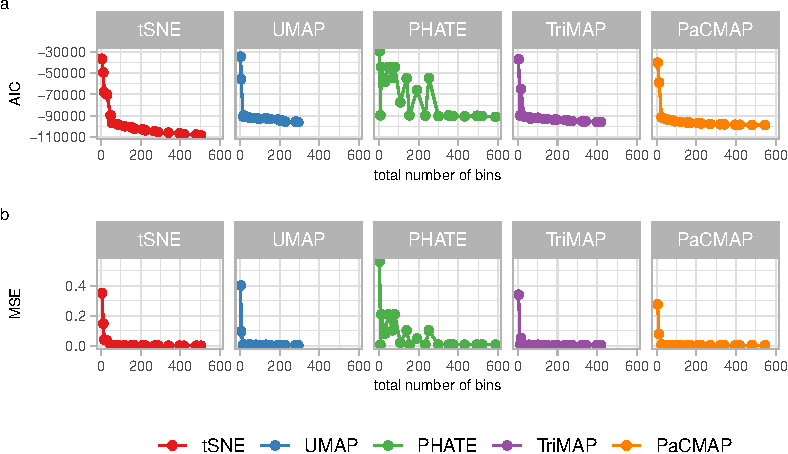
\includegraphics[width=1\textwidth,height=\textheight]{paper_files/figure-pdf/fig-diagnosticpltGau-1.pdf}

}

\caption{\label{fig-diagnosticpltGau}Goodness of fit statistics from
different NLDR techniques applied to training five spherical Gaussian
cluster dataset. What is the best NLDR technique to represent the
original data in 2D?}

\end{figure}

\hypertarget{sec-applications}{%
\section{Applications}\label{sec-applications}}

\hypertarget{single-cell-rna-seq-data-of-human}{%
\subsection{Single-cell RNA-seq data of
human}\label{single-cell-rna-seq-data-of-human}}

In the field of single-cell studies, a common analysis task involves
clustering to identify groups of cells with similar expression profiles.
Analysts often turn to NLDR techniques to verify and identify these
clusters and explore developmental trajectories. In clustering
workflows, the main objective is to verify the existence of clusters and
subsequently identify them as specific cell types by examining the
expression of ``known'' marker genes. Marker genes are specific genes or
transcripts that are uniquely or highly expressed in particular cell
types. Marker genes are identified through differential gene expression
(DEG) analysis, comparing the expression levels of genes across
different cell types. In this context, a ``faithful'' embedding should
ideally preserve the topology of the data, ensuring that cells
corresponding to the same cell type are situated close to the
high-dimensional space.

\hypertarget{processing-steps}{%
\subsection{Processing steps}\label{processing-steps}}

To begin our analysis, we installed the Peripheral Blood Mononuclear
Cells (pbmc) data set obtained from 10x Genomics using the
\texttt{SeuratData} R package \citep{Rahul2019}, which facilitates the
distribution of data sets in the form of Seurat objects
\citep{Yuhan2021}. This data set contains 13,714 features (genes) across
2,700 samples (cells) within a single assay. The active assay is RNA,
with 13,714 features representing different gene expressions. Then, the
cells that have unique feature counts over 2,500 or less than 200 and
cells that have \textgreater{} 5\% mitochondrial counts are filtered.
After removing unwanted cells from the dataset, the next step is to
normalize the data. By default, we employ a global-scaling normalization
method ``LogNormalize'' that normalizes the feature expression
measurements for each cell by the total expression, multiplies this by a
scale factor (10,000 by default), and log-transforms the result.

Next, top 1000 genes are selected by Festem \citep{Chen2023} DEG method.
Then, scale the data. Then, perform PCA on the scaled data. Louvain
algorithm is used to cluster the single cells based on the genes
selected by Festem. Using the Festem-selected genes and 15 PCs,
identified 10 clusters in the PBMC3k data and annotated them based on
the expression of canonical markers. The 10 clusters included immune
cells such as naive CD4 T cells, memory CD4 T cells, CD8 T cells, CD14
monocytes, FCGR3A monocytes, Natural Killer (NK) cells, B cells and
Dendritic Cells (DC). In addition to these common cell types, Festem
identified a fine cell type, CD27− CD4+ memory T cells, which were often
missed by other methods.

\begin{itemize}
\item
  Human peripheral blood mononclear cells (PBMCs) data
\item
  Intro to the data set
\end{itemize}

Used Louvain algorithm to cluster the single cells based on the genes
selected by Festem method

\begin{itemize}
\item
  Explain what ``Evaluate Festem on DEG detection'' means, in terms of
  this data
\item
  How did they ``identified 10 clusters''? What were the variables used,
  PCs or full data or 2D representation, spell this out.
\item
  Used top 1000 genes selected by Festem to run PCA, top 15 PCs
  (original paper mentioned)
\item
  The ``10 clusters included immune cells such as naive CD4 T \ldots{}''
  does this mean that every cluster had all of these, or one cluster was
  mostly ``CD4 T cells'', another mostly ``memory CD4 T'', \ldots?
\item
  How is your use of this data different from the original application.
\item
  Original paper used this data set to compare different DEG methods,
  but we need to look how the performance of UMAP with the author's
  selected parameter choice.
\item
  Why 15 PCs? Is that from the original paper? YES
\end{itemize}

\citet{Chen2023}

\begin{itemize}
\item
  Intro to the data set (This data set contains 13,714 features across
  2,700 samples within a single assay. The active assay is RNA, with
  13,714 features representing different gene expressions.)
\item
  2622 cells
\item
  Evaluate Festem on DEG detection (Festem enabled identification of
  often-missed fine cell types)
\item
  Using the Festem-selected genes, identified 10 clusters in the PBMCsk
  data and annotated them based on the expression of canonical markers
\item
  The 10 clusters included immune cells such as naive CD4 T cells,
  memory CD4 T cells, CD8 T cells, CD14 monocytes, FCGR3A monocytes,
  Natural Killer (NK) cells, B cells and Dendritic Cells (DC).
\item
  In addition to these common cell types, Festem identified a fine cell
  type, CD27− CD4+ memory T cells, which were often missed by other
  methods.
\item
  The CD27. CD4+ memory T cells identified by Festem expressed common
  marker genes (IL7R and S100A4) of memory T cells, but did not express
  CD27. These cells also had downregulated expression of SELL, CCR7, MAL
  and LEF1, and upregulated expression of CCL5 (Fig. 4B) and thus were
  the CD27- CD4+ memory T cells in the literature (36). The CD27- CD4+
  memory T cells were known to be at a more differentiated state and
  have stronger antigen-recall responses than their CD27+ counterparts.
\item
  15 PCs
\item
  Num bins along the x-axis = 23, shape parameter = 0.8772751
\item
  learned from the model: There are 3 well-separated clusters in 2D, but
  if look at the model in high-D space, the three clusters are much
  closer. Also, there is some continuity within the clustering structure
  and it didn't capture well. Therefore UMAP with n:neighbour 30 is not
  a good representation for this data set.
\item
  The most important parameter is n\_neighbors - the number of
  approximate nearest neighbors used to construct the initial
  high-dimensional graph. It effectively controls how UMAP balances
  local versus global structure - low values will push UMAP to focus
  more on local structure by constraining the number of neighboring
  points considered when analyzing the data in high dimensions, while
  high values will push UMAP towards representing the big-picture
  structure while losing fine detail.
\item
  The second parameter we'll investigate is min\_dist, or the minimum
  distance between points in low-dimensional space. This parameter
  controls how tightly UMAP clumps points together, with low values
  leading to more tightly packed embeddings. Larger values of min\_dist
  will make UMAP pack points together more loosely, focusing instead on
  the preservation of the broad topological structure.
\item
  The third parameter is metric. This parameter plays a crucial role in
  determining how distances are computed within the ambient space of the
  input data (The term ``ambient space'' refers to the original or
  initial space in which the data exists before any transformation or
  dimensionality reduction).
\item
  If it is completely a mess, then that is also further evidence that
  the fit is poor in high-dimensions.
\end{itemize}

\begin{table}[H]

\caption{errors for different parameter combinations}
\centering
\begin{tabular}[t]{r|r|l|r}
\hline
\textbf{n\_neighbors} & \textbf{min\_dist} & \textbf{metric} & \textbf{error (x 100)}\\
\hline
\cellcolor{gray!6}{5} & \cellcolor{gray!6}{0.99} & \cellcolor{gray!6}{cosine} & \cellcolor{gray!6}{262.18}\\
\hline
15 & 0.99 & cosine & 279.49\\
\hline
\cellcolor{gray!6}{84} & \cellcolor{gray!6}{0.99} & \cellcolor{gray!6}{cosine} & \cellcolor{gray!6}{295.64}\\
\hline
5 & 0.30 & cosine & 303.90\\
\hline
\cellcolor{gray!6}{15} & \cellcolor{gray!6}{0.30} & \cellcolor{gray!6}{cosine} & \cellcolor{gray!6}{308.97}\\
\hline
84 & 0.30 & cosine & 319.59\\
\hline
\textcolor{red}{\textbf{\cellcolor{gray!6}{30}}} & \textcolor{red}{\textbf{\cellcolor{gray!6}{0.30}}} & \textcolor{red}{\textbf{\cellcolor{gray!6}{cosine}}} & \textcolor{red}{\textbf{\cellcolor{gray!6}{386.35}}}\\
\hline
\end{tabular}
\end{table}

\begin{figure}

{\centering 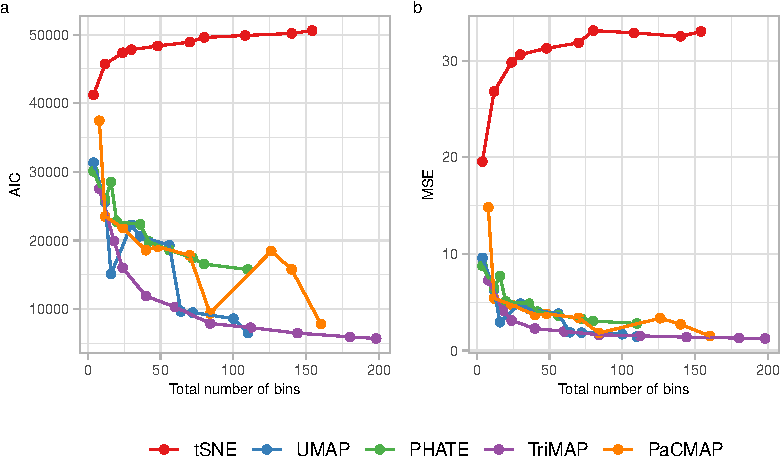
\includegraphics{paper_files/figure-pdf/fig-diagnosticpltPBMC-1.pdf}

}

\caption{\label{fig-diagnosticpltPBMC}Goodness of fit statistics from
UMAP applied to training S-curve dataset. What is the effective number
of bins in each NLDR technique to create a 2D model? The MSE plot have a
steep slope at the beginning, indicating that a smaller number of bins
causes a larger amount of error. Then, the slope gradually declines or
level off, indicating that a higher number of bins generates a smaller
error. Using the elbow method, when the total number of bins is set to
144, the slope of the Mean Squared Error (MSE) plot experiences a sudden
and noticeable change, resembling an elbow-like shape. This point
indicates that adding less bins does not enough to capture the data
structure.}

\end{figure}

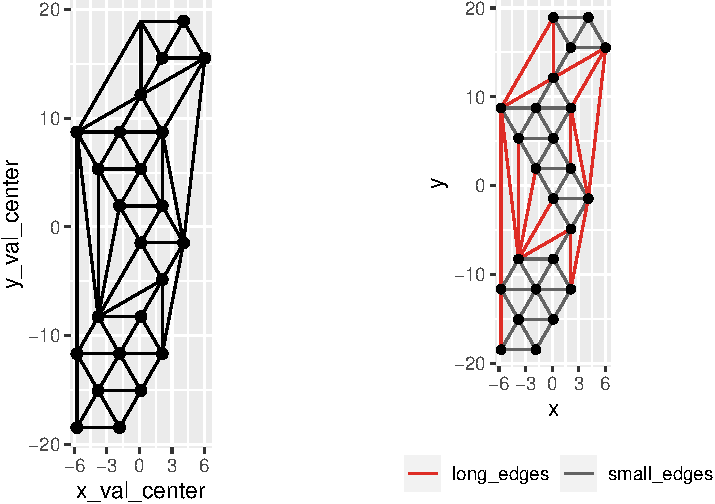
\includegraphics{paper_files/figure-pdf/unnamed-chunk-56-1.pdf}

\begin{figure}[h]

{\centering 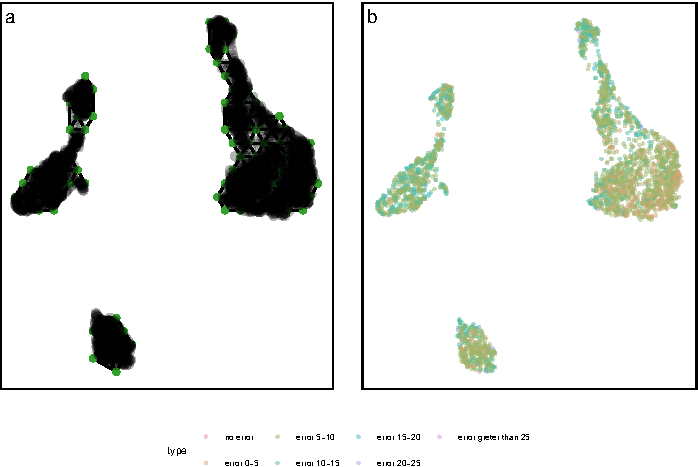
\includegraphics[width=1\textwidth,height=\textheight]{paper_files/figure-pdf/fig-nldervisPBMCUMAP-1.pdf}

}

\caption{\label{fig-nldervisPBMCUMAP}(a) 2D layout from UMAP
(n\_neighbors = 30, min\_dist = 0.3) applied for the PBMC3k dataset. Is
this a best representation of the original data?, (b) Model in the 2D
space with UMAP (\url{https://youtu.be/CNXjWZMyh_M})}

\end{figure}

\begin{figure}

{\centering \includegraphics{paper_files/figure-pdf/fig-diagnosticpltPBMC2-1.pdf}

}

\caption{\label{fig-diagnosticpltPBMC2}Goodness of fit statistics from
UMAP applied to training S-curve dataset. What is the effective number
of bins in each NLDR technique to create a 2D model? The MSE plot have a
steep slope at the beginning, indicating that a smaller number of bins
causes a larger amount of error. Then, the slope gradually declines or
level off, indicating that a higher number of bins generates a smaller
error. Using the elbow method, when the total number of bins is set to
144, the slope of the Mean Squared Error (MSE) plot experiences a sudden
and noticeable change, resembling an elbow-like shape. This point
indicates that adding less bins does not enough to capture the data
structure.}

\end{figure}

\begin{figure}[h]

{\centering \includegraphics[width=1\textwidth,height=\textheight]{paper_files/figure-pdf/fig-nldervisPBMCUMAP2-1.pdf}

}

\caption{\label{fig-nldervisPBMCUMAP2}(a) 2D layout from UMAP
(n\_neighbors = 15, min\_dist = 0.99, metric = cosine) applied for the
PBMC3k dataset. Is this a best representation of the original data?, (b)
Model in the 2D space with UMAP (\textless\textgreater)}

\end{figure}

\begin{figure}

{\centering \includegraphics{paper_files/figure-pdf/fig-diagnosticpltPBMC3-1.pdf}

}

\caption{\label{fig-diagnosticpltPBMC3}Goodness of fit statistics from
UMAP applied to training S-curve dataset. What is the effective number
of bins in each NLDR technique to create a 2D model? The MSE plot have a
steep slope at the beginning, indicating that a smaller number of bins
causes a larger amount of error. Then, the slope gradually declines or
level off, indicating that a higher number of bins generates a smaller
error. Using the elbow method, when the total number of bins is set to
144, the slope of the Mean Squared Error (MSE) plot experiences a sudden
and noticeable change, resembling an elbow-like shape. This point
indicates that adding less bins does not enough to capture the data
structure.}

\end{figure}

\begin{figure}[h]

{\centering \includegraphics[width=1\textwidth,height=\textheight]{paper_files/figure-pdf/fig-nldervisPBMCUMAP3-1.pdf}

}

\caption{\label{fig-nldervisPBMCUMAP3}(a) 2D layout from UMAP
(n\_neighbors = 5, min\_dist = 0.99, metric = cosine) applied for the
PBMC3k dataset. Is this a best representation of the original data?, (b)
Model in the 2D space with UMAP (\textless\textgreater)}

\end{figure}

\hypertarget{harps-gto-sample-dataset}{%
\subsection{HARPS GTO sample dataset}\label{harps-gto-sample-dataset}}

\citet{Anders2018}

\begin{itemize}
\item
  In 2D, there are two well-separated clusters, but the clusters are
  really close
\item
  One cluster have a sparse data space within the cluster
\item
  There is a line in right corner of the structure that is not connected
  any other trimesh points. This line create a long edge in high-D
  space.
\item
  In high-D view, the clusters having some non-linearity patter, which
  is also not captured in tSNE. Therefore, this is not a good choice.
  Also, the two clusters are really near to each other and can't see any
  separation. Also continuity of the structure. Long edges are presence
  also.
\item
  The parameter is, in a sense, a guess about the number of close
  neighbors each point has.
\item
  Num bins along the x-axis = 43, shape parameter = 0.4466309
\end{itemize}

\begin{table}[H]

\caption{errors for different parameter combinations}
\centering
\begin{tabular}[t]{r|r}
\hline
\textbf{perplexity} & \textbf{error (x 100)}\\
\hline
\cellcolor{gray!6}{23} & \cellcolor{gray!6}{0.02}\\
\hline
91 & 0.04\\
\hline
\textcolor{red}{\textbf{\cellcolor{gray!6}{40}}} & \textcolor{red}{\textbf{\cellcolor{gray!6}{1.05}}}\\
\hline
\end{tabular}
\end{table}

\begin{figure}

{\centering \includegraphics{paper_files/figure-pdf/fig-diagnosticpltHARPS-1.pdf}

}

\caption{\label{fig-diagnosticpltHARPS}Goodness of fit statistics from
UMAP applied to training S-curve dataset. What is the effective number
of bins in each NLDR technique to create a 2D model? The MSE plot have a
steep slope at the beginning, indicating that a smaller number of bins
causes a larger amount of error. Then, the slope gradually declines or
level off, indicating that a higher number of bins generates a smaller
error. Using the elbow method, when the total number of bins is set to
144, the slope of the Mean Squared Error (MSE) plot experiences a sudden
and noticeable change, resembling an elbow-like shape. This point
indicates that adding less bins does not enough to capture the data
structure.}

\end{figure}

\begin{figure}[h]

{\centering \includegraphics{paper_files/figure-pdf/fig-nldervisharpstSNE-1.pdf}

}

\caption{\label{fig-nldervisharpstSNE}(a) 2D layout from tSNE
(perplexity = 40) applied for the HARPS GTO dataset. Is this a best
representation of the original data?, (b) Model in the 2D space with
tSNE (\url{https://youtu.be/jxo_rPyGv9k})}

\end{figure}

\begin{itemize}
\item
  5 clusters shows in 2D
\item
  3 clusters which are really close shows in high\_d data with the model
\end{itemize}

\begin{figure}

{\centering \includegraphics{paper_files/figure-pdf/fig-diagnosticpltHARPS2-1.pdf}

}

\caption{\label{fig-diagnosticpltHARPS2}Goodness of fit statistics from
UMAP applied to training S-curve dataset. What is the effective number
of bins in each NLDR technique to create a 2D model? The MSE plot have a
steep slope at the beginning, indicating that a smaller number of bins
causes a larger amount of error. Then, the slope gradually declines or
level off, indicating that a higher number of bins generates a smaller
error. Using the elbow method, when the total number of bins is set to
144, the slope of the Mean Squared Error (MSE) plot experiences a sudden
and noticeable change, resembling an elbow-like shape. This point
indicates that adding less bins does not enough to capture the data
structure.}

\end{figure}

\begin{figure}[h]

{\centering \includegraphics{paper_files/figure-pdf/fig-nldervisharpstSNE2-1.pdf}

}

\caption{\label{fig-nldervisharpstSNE2}(a) 2D layout from tSNE
(perplexity = 23) applied for the HARPS GTO dataset. Is this a best
representation of the original data?, (b) Model in the 2D space with
tSNE (\url{https://youtu.be/VO_4SJEoAUA})}

\end{figure}

\begin{figure}

{\centering \includegraphics{paper_files/figure-pdf/fig-diagnosticpltHARPS3-1.pdf}

}

\caption{\label{fig-diagnosticpltHARPS3}Goodness of fit statistics from
UMAP applied to training S-curve dataset. What is the effective number
of bins in each NLDR technique to create a 2D model? The MSE plot have a
steep slope at the beginning, indicating that a smaller number of bins
causes a larger amount of error. Then, the slope gradually declines or
level off, indicating that a higher number of bins generates a smaller
error. Using the elbow method, when the total number of bins is set to
144, the slope of the Mean Squared Error (MSE) plot experiences a sudden
and noticeable change, resembling an elbow-like shape. This point
indicates that adding less bins does not enough to capture the data
structure.}

\end{figure}

\begin{figure}[h]

{\centering \includegraphics{paper_files/figure-pdf/fig-nldervisharpstSNE3-1.pdf}

}

\caption{\label{fig-nldervisharpstSNE3}(a) 2D layout from tSNE
(perplexity = 91) applied for the HARPS GTO dataset. Is this a best
representation of the original data?, (b) Model in the 2D space with
tSNE (\url{https://youtu.be/vLvRfcogft8})}

\end{figure}

\hypertarget{sec-conclusion}{%
\section{Conclusion}\label{sec-conclusion}}

We introduce a new tool to help to determine which method, which
parameter choice provide the most useful representation of high-D data.

\hypertarget{references}{%
\section*{References}\label{references}}
\addcontentsline{toc}{section}{References}

\renewcommand{\bibsection}{}
\bibliography{bibliography.bib}

\newpage{}




\end{document}
